\documentclass[letterpaper,11pt]{article}
\usepackage[T1]{fontenc}
\usepackage[utf8]{inputenc}
\usepackage{lmodern}
\usepackage{amsmath}
\usepackage{amsfonts}
\usepackage{amssymb}
\usepackage{amsthm}
\usepackage{graphicx}
\usepackage{color}
\usepackage{xcolor}
\usepackage{url}
\usepackage{textcomp}
\usepackage{parskip}
\graphicspath{ {../images/} }

\title{MLT Week-3}
\author{Sherry Thomas \\ 21f3001449}

\begin{document}
\maketitle
\tableofcontents

\begin{abstract}
The week commences with an introduction to the concept of clustering and a comprehensive examination of the K-means algorithm, a crucial element within the topic. The week also delves into the constraints of the K-means approach and offers potential remedial measures to address such limitations.
\end{abstract}

\newpage

\section{Introduction to Clustering}
Clustering is a method of unsupervised machine learning that groups similar objects into clusters, discovering structure in data for exploratory analysis or as a pre-processing step for other algorithms. \\
Our objective is to group $n$ datapoints into $k$ clusters. \\
\underline{Notation}:
$$
\{x_1, x_2, \dots, x_n \} \hspace{6em} x_i \in \mathbb{R}^d 
$$
$$
\{z_1, z_2, \dots, z_n\} \hspace{2em} z_i \in \{1, 2, \dots, k\}
$$
\underline{Objective Function}:
$$
F(z_1, z_2, \dots, z_n) = \sum _{i=1} ^{n} {|| x_i - \mu _{z_i} ||}_2 ^2
$$
where
$$
\mu _k = \frac{\displaystyle \sum _{i = 1} ^{n} {x_i \cdot \mathbf{1}(z_i=k)}}{\displaystyle \sum _{i = 1} ^{n} {\mathbf{1}(z_i=k)}}
$$
\underline{Goal}:
$$
\min _{\{z_1, z_2, \ldots, z_n\}} \sum _{i=1} ^{n} {|| x_i - \mu _{z_i} ||}^2
$$
Unfortunately, finding a solution manually is an NP-Hard problem due to the existence of $k^n$ possibilities. As a result, alternative approaches must be considered to address this challenge.


\section{K-means Clustering (Lloyd's Algorithm)}
Lloyd's Algorithm, also known as the k-means algorithm, is a widely used and straightforward method for clustering that divides a dataset into $K$ pre-determined clusters by iteratively computing the mean distance between the points and their cluster centroids.

\newpage
\subsection{The Algorithm}

The algorithm is as follows:

\underline{Step 1: Initialization} \\
Assign $z_1^0, z_2^0, \ldots, z_n^0$ where $z_i^0 \in \{1, 2, \ldots, k\}$. The approach on how to initialize them is discussed later.
    
\underline{Step 2: Compute Means} \\
$$
\mu _k ^t = \frac{\displaystyle \sum _{i = 1} ^{n} {x_i \cdot \mathbf{1}(z_i^t=k)}}{\displaystyle \sum _{i = 1} ^{n} {\mathbf{1}(z_i^t=k)}} \hspace{2em} \forall k
$$
    
\underline{Step 3: Reassignment Step} \\
$$
z _i ^{t+1} = \underset{k}{\arg \min} {|| x_i - \mu _{k} ^t ||}_2 ^2 \hspace{2em} \forall i
$$

\underline{Step 4: Loop until Convergence} \\
Repeat steps 2 and 3 until convergence for $t$ iterations.

\subsection{Fact regarding Lloyd's Algorithm}
Lloyd's Algorithm, also known as K-means, is guaranteed to converge to a solution. While the converged solution may not be the optimal one, it has been observed to produce acceptable clustering results in practice.

\section{Convergence of K-means Algorithm}
The objective function strictly reduces after each reassignment.
$$
F(z_1^{t+1}, z_2^{t+1}, \ldots, z_n^{t+1}) \le F(z_1^{t}, z_2^{t}, \ldots, z_n^{t})
$$
And as there are only finite number of reassignments possible, the algorithm must converge. \\
\underline{Alternate Explanation}: K-means algorithm converges because it is an iterative procedure that minimizes the sum of squared distances between points and their cluster centroids, which is a convex function with a global minimum. The algorithm will reach the convergence point, guaranteed to exist, under mild assumptions on the initial cluster means, making it a reliable tool for clustering.
\newpage

\section{Nature of Clusters Produced by K-means}

Let $\mu _1$ and $\mu _2$ be the centroids of the clusters $C_1$ and $C_2$ respectively. \\
For $C_1$,
\begin{gather*}
    {|| x - \mu _{1} ||}^2 \le {|| x - \mu _{2} ||}^2 \\
    \therefore x^T(\mu _2 - \mu _1) \le \frac{||\mu _2||^2 - ||\mu _1||^2}{2} \hspace{2em} \forall x
\end{gather*}
The cluster regions are known as half-spaces or Voronoi regions.

\begin{figure*} [h]
    \centering
    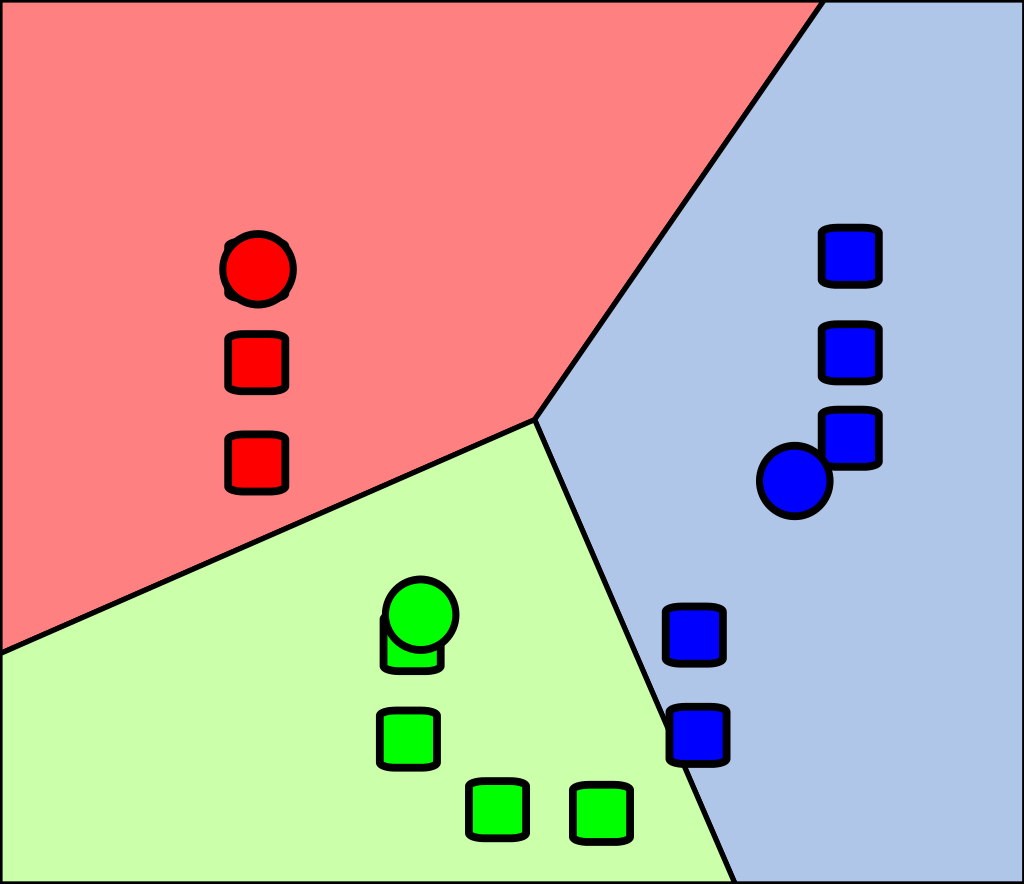
\includegraphics[width=2in]{clustering.png}
    \caption{Voronoi regions for three clusters}
\end{figure*}
But what if the dataset is as follow:

\begin{figure*} [h]
    \centering
    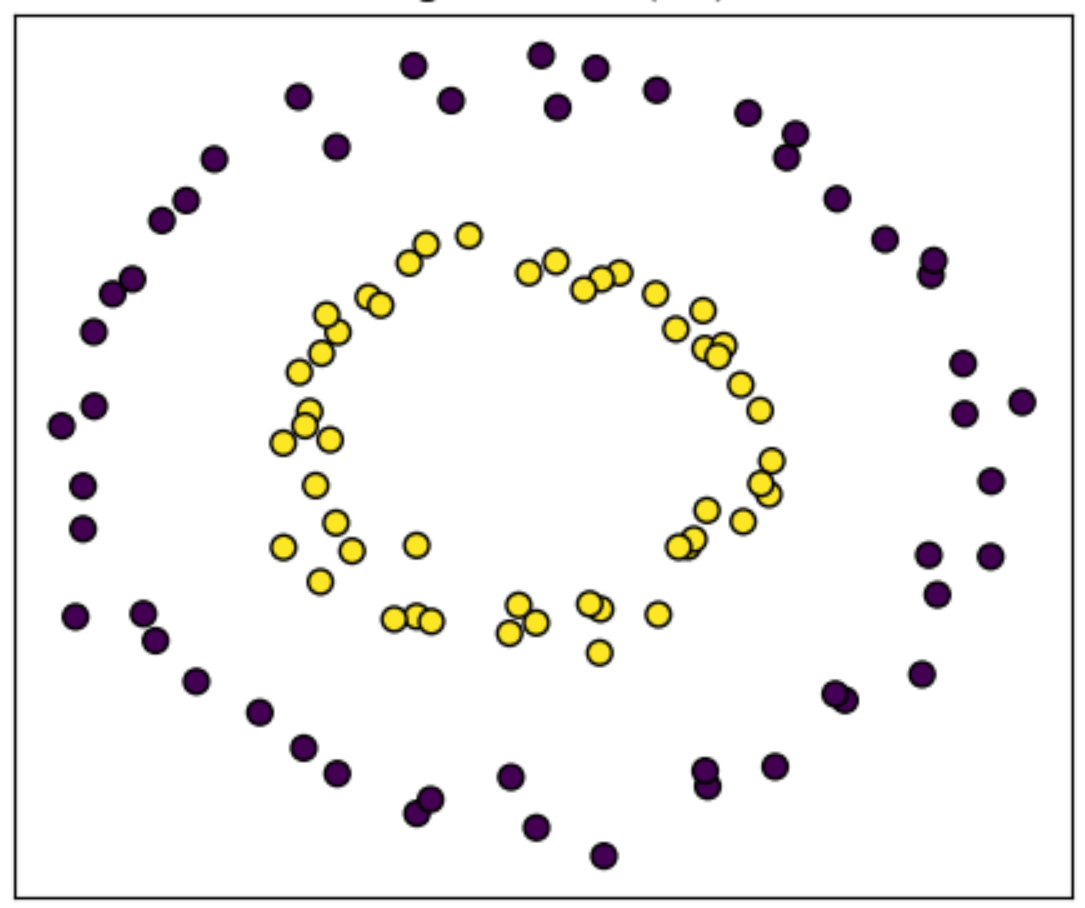
\includegraphics[width=2in]{ccircles.png}
\end{figure*}
The standard k-means algorithm may not perform well when the underlying clusters in the dataset have a non-linear structure. In such cases, alternative methods such as Kernel K-means or Spectral Clustering can be employed to improve clustering accuracy. However, the intricacies of these methods will not be covered in this session.

\section{Initialization of Centroids and K-means++}

One possible way to initialize the centroids is to randomly assign datapoints from the dataset as centroids. \\
The other method is K-means++.
\subsection{K-means++}
The premise is to select centroids that are as far as possible from each other.
\begin{itemize}
    \item Step 1: Choose $\mu _1 ^0$ randomly from the dataset.
    \item Step 2: For $l \in \{2, 3, \ldots, k\}$, choose $\mu _l ^0$ probablistically proportional to score($S$) where $S$ is,
    $$
    S(x) = \min _{\{j=1, 2, \ldots, l-1\}} {|| x - \mu _{j} ^0 ||}^2 \hspace{2em} \forall x
    $$
    The probabilistic aspect of the algorithm provides an expected guarantee of optimal convergence in K-means. The guarantee is given by,
    $$
    \mathbb{E} \left[ \sum _{i=1} ^{n} {|| x_i - \mu _{z_i} ||}^2 \right ]
    \le O(\log k) \left [ \min _{\{z_1, z_2, \ldots, z_n\}} \sum _{i=1} ^{n} {|| x_i - \mu _{z_i} ||}^2 \right ]
    $$
    where $O(\log k)$ is a constant of order $\log k$.
    \item Step 3: Once the centroids are determined, we proceed with Lloyd's Algorithm.
\end{itemize}

\section{Choice of K}
A pre-requisite of K-means is $k$ or the number of clusters. But what if $k$ is unknown? If $k$ is choosen to be equal to $n$,
$$
F(z_1, z_2, \dots, z_n) = \sum _{i=1} ^{n} {|| x_i - \mu _{z_i} ||} ^2 = 0
$$
But we don't want as many clusters as datapoints. Therefore, $k$ needs to be as small as possible. We do this by penalizing large values of k.
$$
\underset{k}{\arg \min} \left [ \sum _{i=1} ^{n} {|| x_i - \mu _{z_i} ||} ^2 + \text{Penalty}(k) \right ]
$$

\newpage
Two common criteria for making the above argument:
\begin{itemize}
    \item Akaike Information Criterion: $\left [ 2K - 2\ln(\hat{\mathcal{L}}(\theta ^*)) \right ]$
    \item Bayesian Information Criterion: $\left [ K\ln(n) - 2\ln(\hat{\mathcal{L}}(\theta ^*)) \right ]$
\end{itemize}
Details for the same will be discussed in future lectures.
 
\section{Credits}
\begin{itemize}
    \item Professor Arun Rajkumar: The content as well as the notations are from his slides and lecture.
\end{itemize}

\end{document}
